\section{Bakti Qilan Mufid}
\subsection{Soal 1}
Buatlah fungsi (file terpisah/library dengan nama \verb|NPM_realtime.py|) untuk mendapatkan data langsung dari arduino

\lstinputlisting[firstline=9, lastline=16]{src/5/1174083/Praktek/1174083_realtime.py}
\begin{figure}[ht!]
	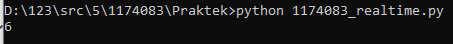
\includegraphics[width=5cm]{figures/5/1174083/Praktek/1.png}
	\centering
	\caption{Membaca Serial tanpa loop}
\end{figure}

\subsection{Soal 2}
Buatlah fungsi (file terpisah/library dengan nama \verb|NPM_save.py|) untuk mendapatkan data langsung dari arduino dengan looping

\lstinputlisting[firstline=10, lastline=18]{src/5/1174083/Praktek/1174083_save.py}


\subsection{Soal 3}
Buatlah fungsi (file terpisah/library dengan nama \verb|NPM_realtime.py|) untuk mendapatkan data dari arduino dan langsung ditulis kedalam file csv
\lstinputlisting[caption="Kode python",firstline=18, lastline=26]{src/5/1174083/Praktek/1174083_realtime.py}
\lstinputlisting[caption="Data yang telah ditulis ke file csv",firstline=0, lastline=10]{src/5/1174083/Praktek/1174083.csv}



\subsection{Soal 4}
Buatlah fungsi (file terpisah/library dengan nama \verb|NPM_csv.py|) untuk membaca file csv hasil arduino dan mengembalikan ke fungsi

\lstinputlisting[firstline=10, lastline=18]{src/5/1174083/Praktek/1174083_csv.py}

\subsection{Ketrampilan Penanganan Error}
Tuliskan peringatan error yang didapat dari mengerjakan praktek ketiga ini, dan jelaskan cara penanganan error tersebut. dan Buatlah satu fungsi yang menggunakan gunakan try except untuk menanggulangi error tersebut.
\begin{itemize}
\item Syntax Errors

Syntax Errors adalah kesalahan pada penulisan syntax atau kode. Solusinya adalah memperbaiki penulisan syntax atau kode

\item Zero Division Error

ZeroDivisonError adalah exceptions yang terjadi saat eksekusi program menghasilkan perhitungan matematika pembagian dengan angka nol (0). Solusinya adalah tidak membagi suatu yang hasilnya nol.

\item Name Error

NameError adalah exception saat kode melakukan eksekusi terhadap local name atau global name yang tidak terdefinisi atau tidak ada. Solusinya adalah memastikan variabel atau function yang akan dipanggil ada didalam program atau tidak salah mengetikannya.

\item Type Error

TypeError adalah exception saat melakukan eksekusi terhadap suatu operasi atau fungsi dengan type object yang tidak sesuai. Solusinya adalah mengkoversi varibelnya sesuai dengan tipe data sesuai dengan yang akan digunakan.

\end{itemize}
\lstinputlisting[firstline=7, lastline=22]{src/5/1174083/Praktek/1174083_error.py}

%%%%%%%%%%%%%%%%%%%%%%%%%%%%%%%%%%%%%%%%%%%%%%%%%%%%%%%%%%%%%%%%%%%%%%%%%%%%%%%%

\section{Muhammad Reza Syachrani / 1174084}
\subsection{Ketrampilan Pemrograman}
\subsubsection{Soal 1}
jawaban : \lstinputlisting[caption=Jawaban no.1, firstline=8, lastline=15, ]{src/5/1174084/Praktek/1174084_realtime.py}

\subsubsection{Soal 2}
jawaban : \lstinputlisting[caption=Jawaban no.2, firstline=8, lastline=16, ]{src/5/1174084/Praktek/1174084_save.py}

\subsubsection{Soal 3}
jawaban : \lstinputlisting[caption=Jawaban no.3, firstline=18, lastline=27, ]{src/5/1174084/Praktek/1174084_realtime.py}

\subsubsection{Soal 4}
jawaban : \lstinputlisting[caption=Jawaban no.4, firstline=8, lastline=16, ]{src/5/1174084/Praktek/1174084_csv.py}

\subsection{Ketrampilan Penanganan Error}

Tuliskan peringatan error yang didapat dari mengerjakan praktek ketiga ini, dan jelaskan cara penanganan error tersebut. dan Buatlah satu fungsi yang menggunakan gunakan try except untuk menanggulangi error tersebut.
\begin{itemize}
\item Syntax Errors

Syntax Errors adalah kesalahan pada penulisan syntax atau kode. Solusinya adalah memperbaiki penulisan syntax atau kode

\item Zero Division Error

ZeroDivisonError adalah exceptions yang terjadi saat eksekusi program menghasilkan perhitungan matematika pembagian dengan angka nol (0). Solusinya adalah tidak membagi suatu yang hasilnya nol.

\item Name Error

NameError adalah exception saat kode melakukan eksekusi terhadap local name atau global name yang tidak terdefinisi atau tidak ada. Solusinya adalah memastikan variabel atau function yang akan dipanggil ada didalam program atau tidak salah mengetikannya.

\item Type Error

TypeError adalah exception saat melakukan eksekusi terhadap suatu operasi atau fungsi dengan type object yang tidak sesuai. Solusinya adalah mengkoversi varibelnya sesuai dengan tipe data sesuai dengan yang akan digunakan.

\end{itemize}
\lstinputlisting[caption=error, firstline=8, lastline=23, ]{src/5/1174084/Praktek/1174084_error.py}
%%%%%%%%%%%%%%%%%%%%%%%%%%%%%%%%%%%%%%%%%%%%%%%%%%%%%%%%%%%%%%%%%%%%%%%%%%%%%%%%%%%%%%
\section{Ilham Muhammad Ariq}
\subsection{Keterampilan Pemrograman}
\begin{enumerate}
	\item Buatlah  fungsi  (file  terpisah/library  dengan  nama  \verb|NPM_realtime.py|)  untuk mendapatkan data langsung dari arduino!

	\lstinputlisting[firstline=8, lastline=14]{src/5/1174087/Praktek/1174087_realtime.py}
	
	\item Buatlah fungsi (file terpisah/library dengan nama \verb|NPM_save.py|) untuk mendapatkan data langsung dari arduino dengan looping!
	
	\lstinputlisting[firstline=8, lastline=15]{src/5/1174087/Praktek/1174087_save.py}

\begin{figure}[ht]
	\includegraphics[width=7cm]{figures/5/1174087/Praktek/1174087_save.png}
	\centering
	\caption{Hasil dari pembacaan fungsi untuk membaca file csv hasil arduino dan mengembalikan fungsi.}
\end{figure}

	\item Buatlah  fungsi  (file  terpisah/library  dengan  nama  \verb|NPM_realtime.py|) untuk mendapatkan data dari arduino dan langsung ditulis kedalam file csv!
	
	\lstinputlisting[firstline=16, lastline=28]{src/5/1174087/Praktek/1174087_realtime.py}

	\item Buatlah fungsi (file terpisah/library dengan nama \verb|NPM_csv.py|) untuk membaca file csv hasil arduino dan mengembalikan ke fungsi!
	
	\lstinputlisting[firstline=8, lastline=14]{src/5/1174087/Praktek/1174087_csv.py}

\end{enumerate}

\textbf{Kode Program Praktek}
\begin{figure}[ht]
	\includegraphics[width=7cm]{figures/5/1174087/Praktek/1174087_realtime.png}
	\centering
\end{figure}

\begin{figure}[ht]
	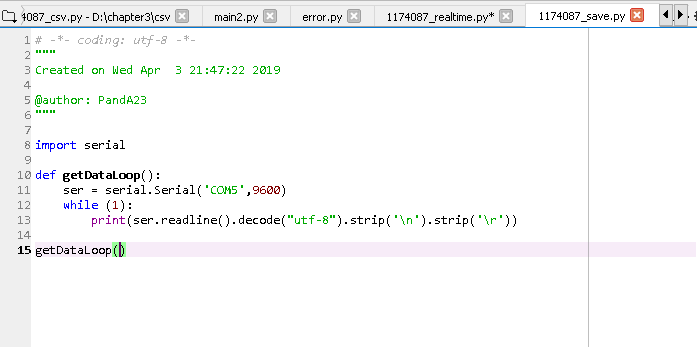
\includegraphics[width=7cm]{figures/5/1174087/Praktek/1174087_save1.png}
	\centering
\end{figure}

\begin{figure}[ht]
	\includegraphics[width=7cm]{figures/5/1174087/Praktek/1174087_csv.png}
	\centering
\end{figure}

\begin{figure}[ht]
	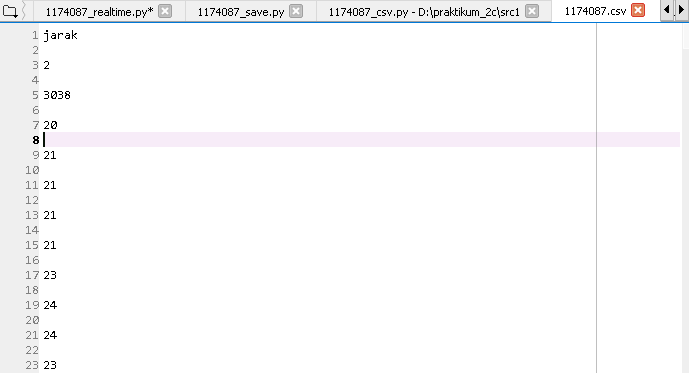
\includegraphics[width=7cm]{figures/5/1174087/Praktek/1174087csv.png}
	\centering
\end{figure}


\subsection{Ketrampilan Penanganan Error}
Tuliskan  peringatan  error  yang  didapat  dari  mengerjakan  praktek  kelima  ini, dan  jelaskan  cara  penanganan  error  tersebut.   dan  Buatlah  satu  fungsi  yang menggunakan try except untuk menanggulangi error tersebut.

Peringatan error di praktek kelima ini, yaitu:
\begin{itemize}
	\item Syntax Errors
	Syntax Errors adalah suatu keadaan saat kode python mengalami kesalahan penulisan. Solusinya adalah memperbaiki penulisan kode yang salah.

	\item Name Error
	NameError adalah exception yang terjadi saat kode melakukan eksekusi terhadap local name atau global name yang tidak terdefinisi. Solusinya adalah memastikan variabel atau function yang dipanggil ada atau tidak salah ketik.

	\item Type Error
	TypeError adalah exception yang akan terjadi apabila pada saat dilakukannya eksekusi terhadap suatu operasi atau fungsi dengan type object yang tidak sesuai. Solusi dari error ini adalah mengkoversi varibelnya sesuai dengan tipe data yang akan digunakan.
\end{itemize}

\textbf{Fungsi yang menggunakan try except untuk menanggulangi error.}

\lstinputlisting[firstline=8, lastline=23]{src/5/1174087/Praktek/1174087_error.py}

\textbf{Kode Program Penanganan Error}
\begin{figure}[ht]
	\includegraphics[width=7cm]{figures/5/1174087/Praktek/1174087_error.png}
	\centering
\end{figure}
%%%%%%%%%%%%%%%%%%%%%%%%%%%%%%%%%%%%%%%%%%%%%%%%%%%%%%%%%%%%%%%%%%%%%%%%%%%%%%%%%%%%%%%%%%%%%%
\section{Advent Nopele Olansi Damiahan Sihite/ 1174089}
{\Large \textbf{Praktek Pemrograman}}
\subsection{Soal No. 1}
Buatlah  fungsi  (file  terpisah/library  dengan  nama  NPMrealtime.py)  untuk mendapatkan data langsung dari arduino!
\lstinputlisting[caption = Fungsi untuk mendapatkan data dari Arduino., firstline=1, lastline=7]{src/5/1174089/Praktek/1174089realtime.py}

\begin{figure}[H]
	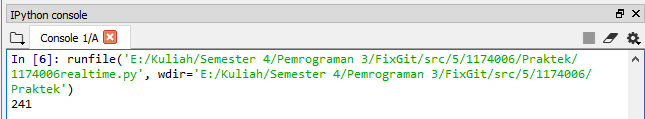
\includegraphics[width=12cm]{figures/5/1174089/Praktek/1.png}
	\centering
	\caption{Hasil dari pembacaan fungsi untuk mendapatkan data dari Arduino.}
\end{figure}

\subsection{Soal No. 2}
Buatlah fungsi (file terpisah/library dengan nama NPMsave.py) untuk mendapatkan data langsung dari arduino dengan looping!
\lstinputlisting[caption = Fungsi untuk mendapatkan data langsung dari Arduino dengan looping., firstline=1, lastline=8]{src/5/1174089/Praktek/1174089save.py}

\begin{figure}[H]
	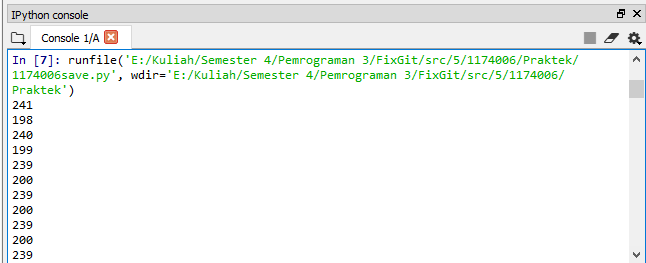
\includegraphics[width=12cm]{figures/5/1174089/Praktek/2.png}
	\centering
	\caption{Hasil dari pembacaan fungsi untuk mendapatkan data dari Arduino dengan looping.}
\end{figure}

\subsection{Soal No. 3}
Buatlah  fungsi  (file  terpisah/library  dengan  nama  NPMrealtime.py) untuk mendapatkan data dari arduino dan langsung ditulis kedalam file csv!
\lstinputlisting[caption = Fungsi untuk mendapatkan data dari Arduino dan langsung ditulis kedalam file CSV., firstline=9, lastline=23]{src/5/1174089/Praktek/1174089realtime.py}

\begin{figure}[H]
	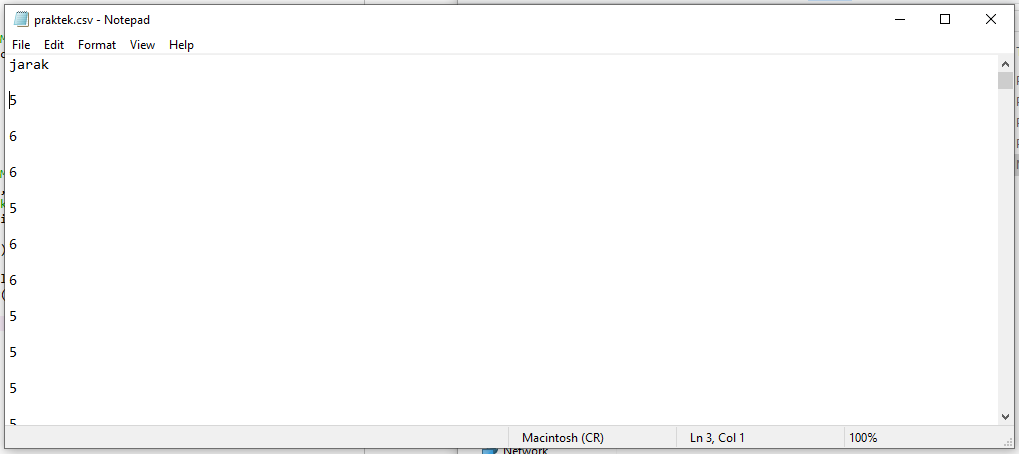
\includegraphics[width=12cm]{figures/5/1174089/Praktek/3.png}
	\centering
	\caption{Hasil dari pembacaan fungsi untuk mendapatkan data dari Arduino dan langsung ditulis kedalam file CSV.}
\end{figure}

\subsection{Soal No. 4}
Buatlah fungsi (file terpisah/library dengan nama NPMcsv.py) untuk membaca file csv hasil arduino dan mengembalikan ke fungsi!
\lstinputlisting[caption = Fungsi untuk membaca file CSV hasil Arduino dan mengembalikan fungsi., firstline=1, lastline=9]{src/5/1174089/Praktek/1174089csv.py}

\begin{figure}[H]
	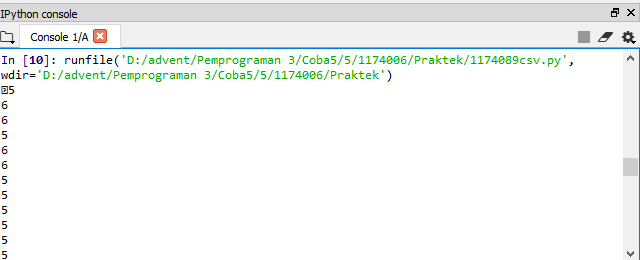
\includegraphics[width=12cm]{figures/5/1174089/Praktek/4.png}
	\centering
	\caption{Hasil dari pembacaan fungsi untuk membaca file csv hasil arduino dan mengembalikan fungsi.}
\end{figure}

\subsection{Kode Program Praktek}
\begin{figure}[H]
	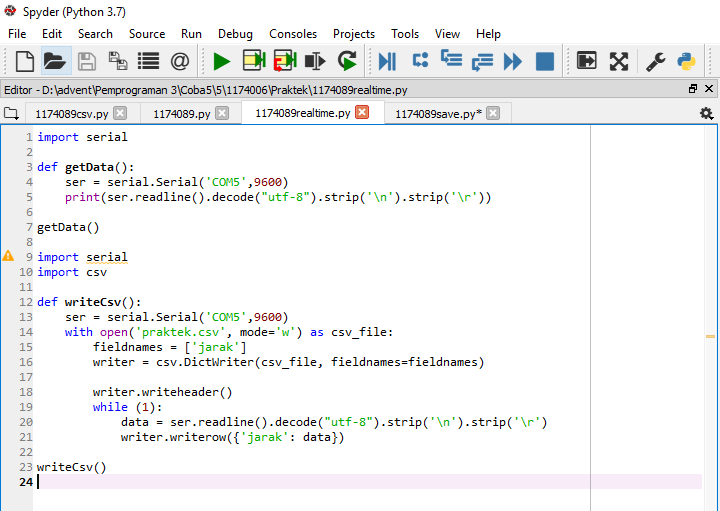
\includegraphics[width=9cm]{figures/5/1174089/Praktek/realtime.png}
	\centering
\end{figure}

\begin{figure}[H]
	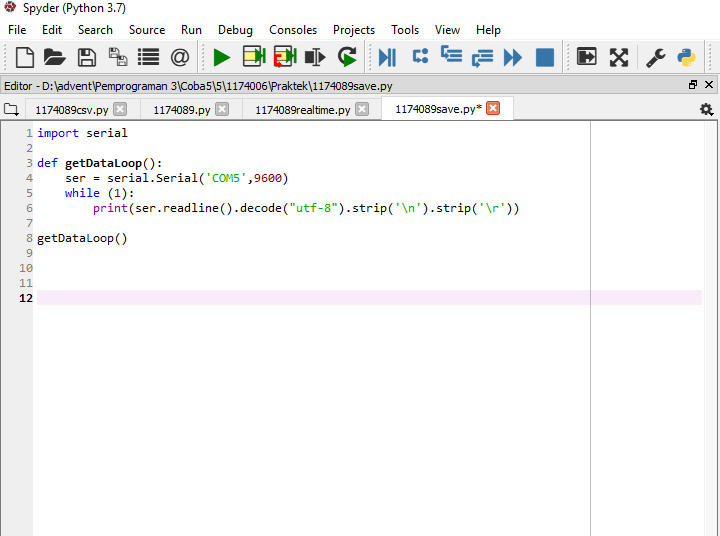
\includegraphics[width=9cm]{figures/5/1174089/Praktek/save.png}
	\centering
\end{figure}

\begin{figure}[H]
	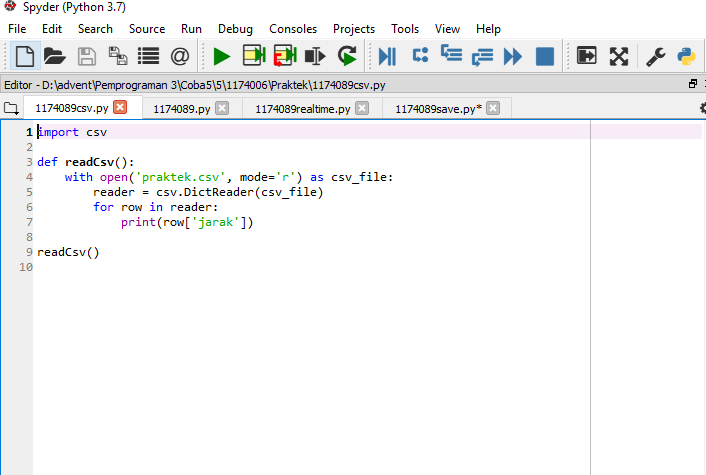
\includegraphics[width=9cm]{figures/5/1174089/Praktek/csv.png}
	\centering
\end{figure}

\subsection{Cek Plagiat Praktek}
\begin{figure}[H]
	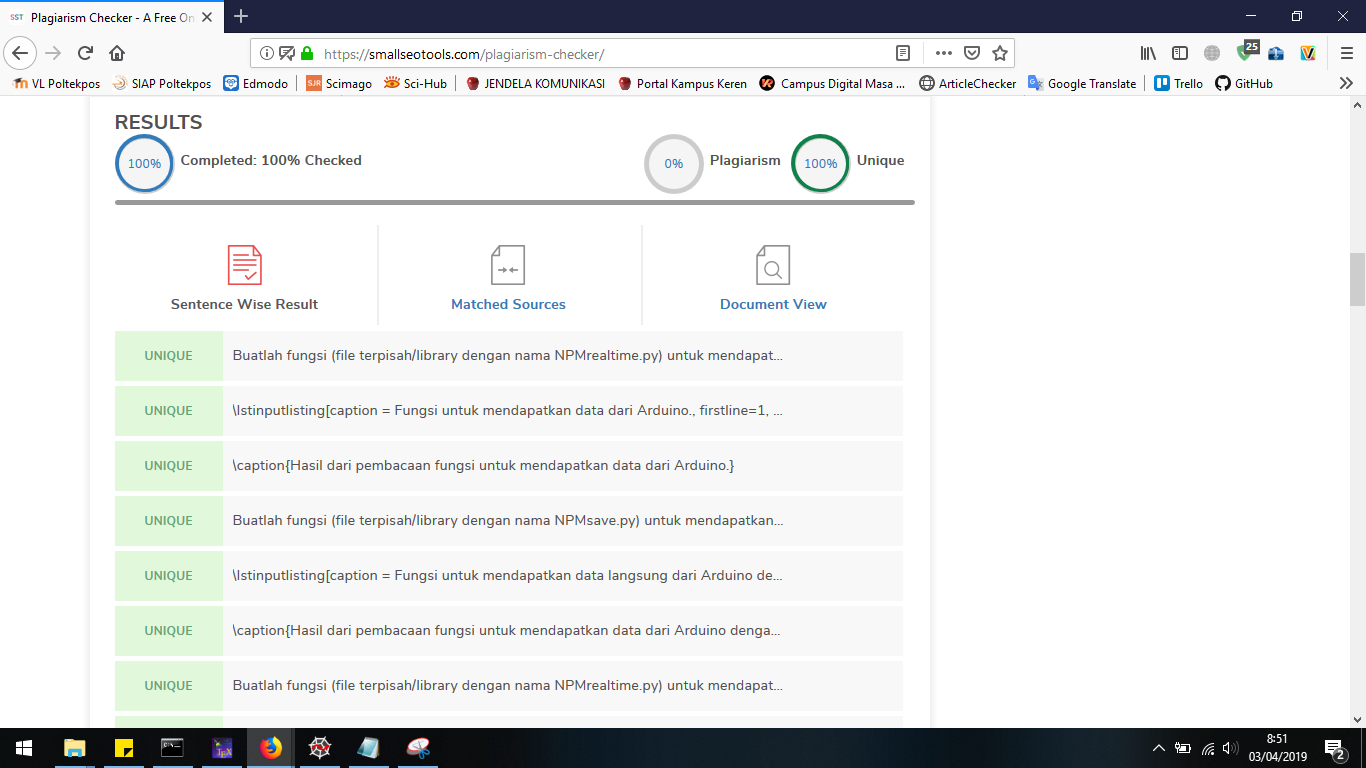
\includegraphics[width=9cm]{figures/5/1174089/Praktek/plagiatpraktek.png}
	\centering
\end{figure}

\hfill \break
{\Large \textbf{Ketrampilan Penanganan Error}}

\subsection{Soal No. 1}
Tuliskan  peringatan  error  yang  didapat  dari  mengerjakan  praktek  kelima  ini, dan  jelaskan  cara  penanganan  error  tersebut.   dan  Buatlah  satu  fungsi  yang menggunakan try except untuk menanggulangi error tersebut.

\hfill \break
Peringatan error di praktek kelima ini, yaitu:
\begin{itemize}
	\item Syntax Errors
	Syntax Errors adalah suatu keadaan saat kode python mengalami kesalahan penulisan. Solusinya adalah memperbaiki penulisan kode yang salah.
	
	\item Name Error
	NameError adalah exception yang terjadi saat kode melakukan eksekusi terhadap local name atau global name yang tidak terdefinisi. Solusinya adalah memastikan variabel atau function yang dipanggil ada atau tidak salah ketik.
	
	\item Type Error
	TypeError adalah exception yang akan terjadi apabila pada saat dilakukannya eksekusi terhadap suatu operasi atau fungsi dengan type object yang tidak sesuai. Solusi dari error ini adalah mengkoversi varibelnya sesuai dengan tipe data yang akan digunakan.
\end{itemize}

\hfill \break
Fungsi yang menggunakan try except untuk menanggulangi error.

\lstinputlisting[caption = Fungsi untuk menanggulangi error menggunakan Try Except., firstline=1, lastline=16]{src/5/1174089/Praktek/1174089.py}

\begin{figure}[H]
	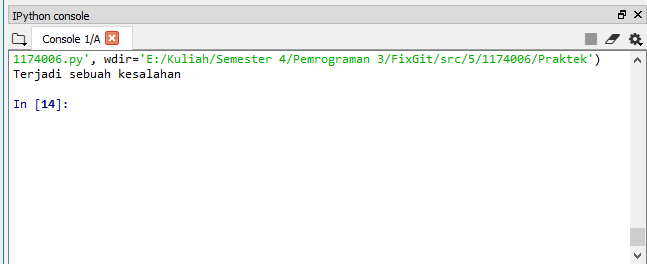
\includegraphics[width=12cm]{figures/5/1174089/Praktek/5.png}
	\centering
	\caption{Hasil pembacaan fungsi untuk menanggulangi error menggunakan Try Except.}
\end{figure}

\subsection{Kode Program Penanganan Error}
\begin{figure}[H]
	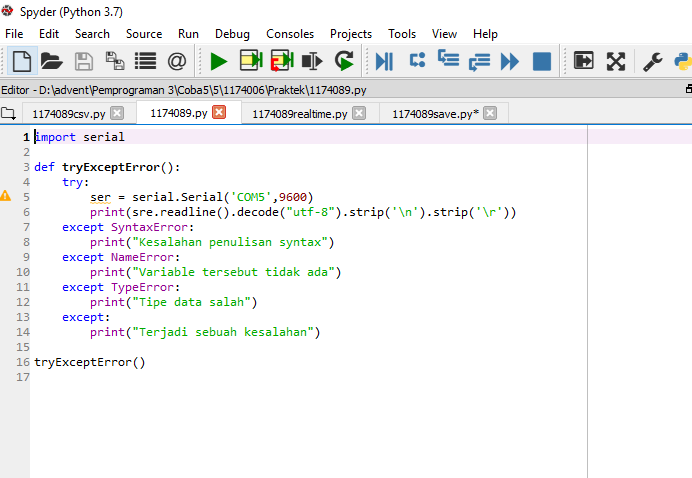
\includegraphics[width=12cm]{figures/5/1174089/Praktek/error.png}
	\centering
\end{figure}

\subsection{Cek Plagiat Penanganan Error}
\begin{figure}[H]
	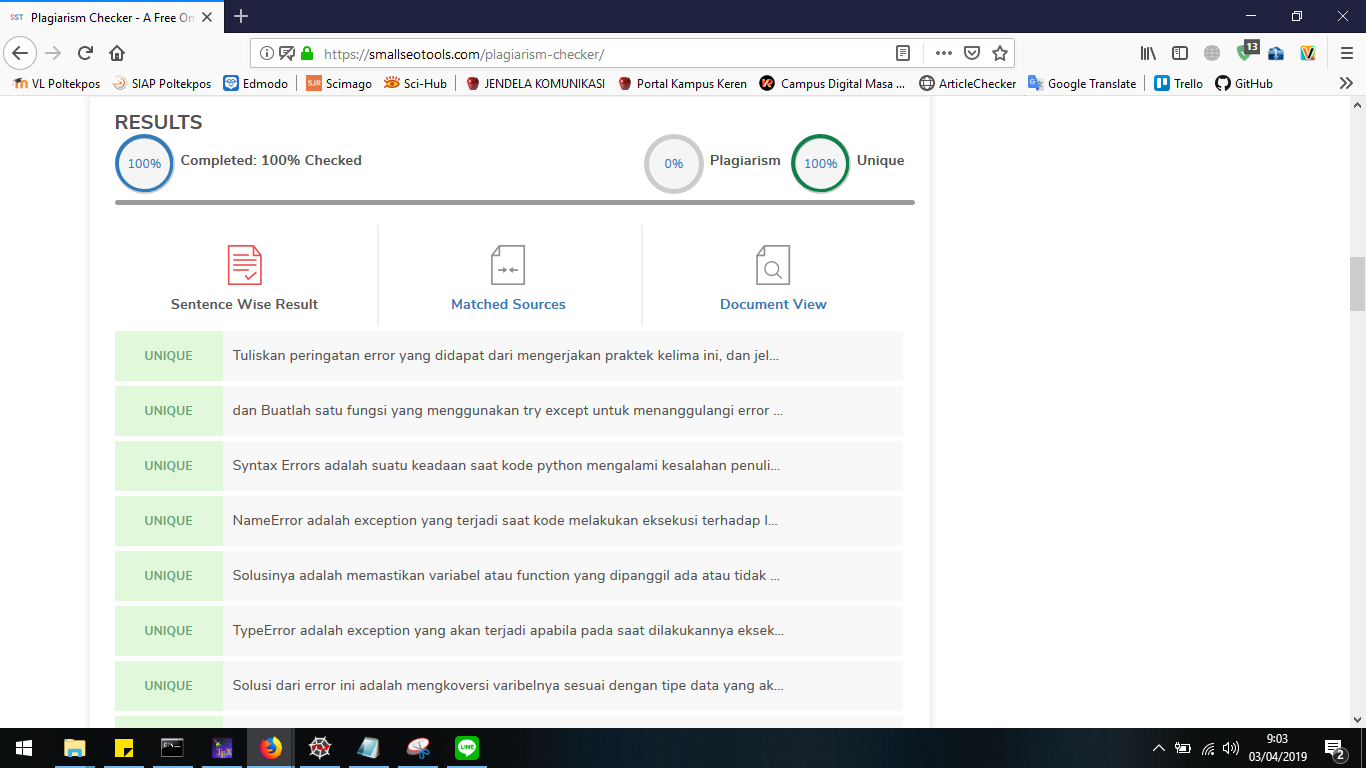
\includegraphics[width=12cm]{figures/5/1174089/Praktek/plagiaterror.png}
	\centering
\end{figure}
%%%%%%%%%%%%%%%%%%%%%%%%%%%%%%%%%%%%%%%%%%%%%%%%%%%%%%%%%%%%%%%%%%%%%%%%%%%%%%%%%%%%%%%%%%%%%%%%%%%%%%
\section{Dini Permata Putri}
\subsection{Keterampilan Pemrograman}
\begin{enumerate}
	\item Buatlah  fungsi  (file  terpisah/library  dengan  nama  \verb|NPM_realtime.py|)  untuk mendapatkan data langsung dari arduino!

	\lstinputlisting[firstline=8, lastline=29]{src/5/1174053/Praktek/1174053_realtime.py}
	
	\item Buatlah fungsi (file terpisah/library dengan nama \verb|NPM_save.py|) untuk mendapatkan data langsung dari arduino dengan looping!
	
	\lstinputlisting[firstline=8, lastline=15]{src/5/1174053/Praktek/1174053_save.py}

\begin{figure}[ht]
	\includegraphics[width=7cm]{figures/5/1174053/Praktek/1174053_save.png}
	\centering
	\caption{Hasil dari pembacaan fungsi untuk membaca file csv hasil arduino dan mengembalikan fungsi.}
\end{figure}

	\item Buatlah  fungsi  (file  terpisah/library  dengan  nama  \verb|NPM_realtime.py|) untuk mendapatkan data dari arduino dan langsung ditulis kedalam file csv!
	
	\lstinputlisting[firstline=8, lastline=29]{src/5/1174053/Praktek/1174053_realtime.py}

	\item Buatlah fungsi (file terpisah/library dengan nama \verb|NPM_csv.py|) untuk membaca file csv hasil arduino dan mengembalikan ke fungsi!
	
	\lstinputlisting[firstline=8, lastline=16]{src/5/1174053/Praktek/1174053_csv.py}

\end{enumerate}

\textbf{Kode Program Praktek}

\subsection{Ketrampilan Penanganan Error}
Tuliskan  peringatan  error  yang  didapat  dari  mengerjakan  praktek  kelima  ini, dan  jelaskan  cara  penanganan  error  tersebut.   dan  Buatlah  satu  fungsi  yang menggunakan try except untuk menanggulangi error tersebut.

Peringatan error di praktek kelima ini, yaitu:
\begin{itemize}
	\item Syntax Errors
	Syntax Errors adalah suatu keadaan saat kode python mengalami kesalahan penulisan. Solusinya adalah memperbaiki penulisan kode yang salah.

	\item Name Error
	NameError adalah exception yang terjadi saat kode melakukan eksekusi terhadap local name atau global name yang tidak terdefinisi. Solusinya adalah memastikan variabel atau function yang dipanggil ada atau tidak salah ketik.

	\item Type Error
	TypeError adalah exception yang akan terjadi apabila pada saat dilakukannya eksekusi terhadap suatu operasi atau fungsi dengan type object yang tidak sesuai. Solusi dari error ini adalah mengkoversi varibelnya sesuai dengan tipe data yang akan digunakan.
\end{itemize}

\textbf{Fungsi yang menggunakan try except untuk menanggulangi error.}

\lstinputlisting[firstline=8, lastline=23]{src/5/1174053/Praktek/1174053_error.py}

\textbf{Kode Program Penanganan Error}
%%%%%%%%%%%%%%%%%%%%%%%%%%%%%%%%%%%%%%%%%%%%%%%%%%%%%%%%%%%%%%%%%%%%%%%%%%%%%%%%%%%%
\section{Mochamad Arifqi Ramadhan | 1174074}
\subsection{Soal 1}
Buatlah fungsi (file terpisah/library dengan nama \verb|NPM_realtime.py|) untuk mendapatkan data langsung dari arduino

\lstinputlisting[firstline=9, lastline=16]{src/5/1174074/Praktek/1174074_realtime.py}


\subsection{Soal 2}
Buatlah fungsi (file terpisah/library dengan nama \verb|NPM_save.py|) untuk mendapatkan data langsung dari arduino dengan looping

\lstinputlisting[firstline=9, lastline=17]{src/5/1174074/Praktek/1174074_save.py}


\subsection{Soal 3}
Buatlah fungsi (file terpisah/library dengan nama \verb|NPM_realtime.py|) untuk mendapatkan data dari arduino dan langsung ditulis kedalam file csv
\lstinputlisting[caption="Kode python",firstline=18, lastline=26]{src/5/1174083/Praktek/1174074_realtime.py}
\lstinputlisting[caption="Data yang telah ditulis ke file csv",firstline=0, lastline=10]{src/5/1174074/Praktek/1174074.csv}


\subsection{Soal 4}
Buatlah fungsi (file terpisah/library dengan nama \verb|NPM_csv.py|) untuk membaca file csv hasil arduino dan mengembalikan ke fungsi

\lstinputlisting[firstline=9, lastline=18]{src/5/1174074/Praktek/1174074_csv.py}

\subsection{Keterampilan Penanganan Error}
Tuliskan peringatan error yang didapat dari mengerjakan praktek ketiga ini, dan jelaskan cara penanganan error tersebut. dan Buatlah satu fungsi yang menggunakan gunakan try except untuk menanggulangi error tersebut.
\begin{itemize}
\item Syntax Errors

Syntax Errors adalah kesalahan pada penulisan syntax atau kode. Solusinya adalah memperbaiki penulisan syntax atau kode

\item Zero Division Error

ZeroDivisonError adalah exceptions yang terjadi saat eksekusi program menghasilkan perhitungan matematika pembagian dengan angka nol (0). Solusinya adalah tidak membagi suatu yang hasilnya nol.

\item Name Error

NameError adalah exception saat kode melakukan eksekusi terhadap local name atau global name yang tidak terdefinisi atau tidak ada. Solusinya adalah memastikan variabel atau function yang akan dipanggil ada didalam program atau tidak salah mengetikannya.

\item Type Error

TypeError adalah exception saat melakukan eksekusi terhadap suatu operasi atau fungsi dengan type object yang tidak sesuai. Solusinya adalah mengkoversi varibelnya sesuai dengan tipe data sesuai dengan yang akan digunakan.

\end{itemize}
\lstinputlisting[firstline=5, lastline=22]{src/5/1174074/Praktek/1174074_error.py}


\textbf{Kode Program Praktek}
\begin{figure}[ht]
	\includegraphics[width=7cm]{figures/5/1174074/Praktek/1174087_realtime.png}
	\centering
\end{figure}

\begin{figure}[ht]
	\includegraphics[width=7cm]{figures/5/1174074/Praktek/1174087_save.png}
	\centering
\end{figure}

\begin{figure}[ht]
	\includegraphics[width=7cm]{figures/5/1174074/Praktek/1174087_csv.png}
	\centering
\end{figure}

\begin{figure}[ht]
	\includegraphics[width=7cm]{figures/5/1174074/Praktek/1174087_error.png}
	\centering
\end{figure}
%%%%%%%%%%%%%%%%%%%%%%%%%%%%%%%%%%%%%%%%%%%%%%%%%%%%%%%%%%%%%%%%%%%%%%%%%%%%%%%%%%%%%%%%%%%%%%%%